\documentclass[11pt,compress,t,notes=noshow, aspectratio=169, xcolor=table]{beamer}

\usepackage{../../style/lmu-lecture}
% Defines macros and environments
% This file is included in slides and exercises

% Rarely used fontstyle for R packages, used only in 
% - forests/slides-forests-benchmark.tex
% - exercises/single-exercises/methods_l_1.Rnw
% - slides/cart/attic/slides_extra_trees.Rnw
\newcommand{\pkg}[1]{{\fontseries{b}\selectfont #1}}

% Spacing helpers, used often (mostly in exercises for \dlz)
\newcommand{\lz}{\vspace{0.5cm}} % vertical space (used often in slides)
\newcommand{\dlz}{\vspace{1cm}}  % double vertical space (used often in exercises, never in slides)
\newcommand{\oneliner}[1] % Oneliner for important statements, used e.g. in iml, algods
{\begin{block}{}\begin{center}\begin{Large}#1\end{Large}\end{center}\end{block}}

% Don't know if this is used or needed, remove?
% textcolor that works in mathmode
% https://tex.stackexchange.com/a/261480
% Used e.g. in forests/slides-forests-bagging.tex
% [...] \textcolor{blue}{\tfrac{1}{M}\sum^M_{m} [...]
% \makeatletter
% \renewcommand*{\@textcolor}[3]{%
%   \protect\leavevmode
%   \begingroup
%     \color#1{#2}#3%
%   \endgroup
% }
% \makeatother


\title{Interpretable Machine Learning}
% \author{LMU}
%\institute{\href{https://compstat-lmu.github.io/lecture_iml/}{compstat-lmu.github.io/lecture\_iml}}
\date{}

\begin{document}

\newcommand{\titlefigure}{figure/h-statistic}
\newcommand{\learninggoals}{
\item Friedman's H-statistic with two purposes:
\item Measure general $k$-way interactions between arbitrary features
\item Measure a single feature's overall interaction strength
}

\lecturechapter{Friedman's H-Statistic}
\lecture{Interpretable Machine Learning}



\begin{frame}{Idea \citebutton{Friedman and Popescu (2008)}{https://doi.org/10.1214/07-AOAS148}}

    \textbf{2-way interaction:}
    \begin{itemize}[<+->]
        \item Two features $j$ and $k$ do not interact, if their 2-way interaction component in functional decomposition $g_{\{j,k\}}$ is 0
        \item Idea from standard fANOVA: PD-function contains all components:
        $$
        \fh_{\{jk\}, PD}(x_j, x_k)
        = g_\emptyset + g_j(x_j) + g_k(x_k) + g_{\{j,k\}}(x_j, x_k)
        $$
        \item Here: \textbf{Centered PD-functions} $\fh_{S,PD}^c(\xv_S) = \fh_{S,PD}(\xv_S) - g_\emptyset$
        $$
        \Rightarrow \fh^c_{\{jk\}, PD}(x_j, x_k)
        = g_j(x_j) + g_k(x_k) + g_{\{j,k\}}(x_j, x_k)
        $$
        \item \textbf{Definition:} A function $\fh$ contains no 2-way interactions between $j$ and $k$, if there exists a decomposition
        \begin{align*}
            % & \fh_{\{jk\}, PD}(x_j, x_k)
            % = g_\emptyset + g_j(x_j) + g_k(x_k) \\
            % \Leftrightarrow \quad
            & \fh_{\{jk\}, PD}^c(x_xj, x_k)
            = g_j(x_j) + g_k(x_k) \\
            \Leftrightarrow \quad
            & \fh_{\{jk\}, PD}^c(x_j, x_k)
            = \fh^c_{j, PD}(x_j) + \fh^c_{k, PD}(x_k)
        \end{align*}
        \item This means: There are interactions \\
        $\Leftrightarrow$ Every possible decomposition must contain some non-zero term $g_{\{j,k\}}(x_j, x_k)$
        \item Again: remember GAMs
    \end{itemize}
    
% 	$$\fh_{jk, PD}(x_j, x_k) = \fh_{j, PD}(x_j) + \fh_{k, PD}(x_k)$$

% \begin{itemize}
% 	\item $\fh_{jk, PD}(x_j, x_k)$: joint 2-dim PD function of feature $j$ and $k$
% 	\item $\fh_{j, PD}(x_j)$ and $\fh_{k, PD}(x_k)$: 1-dim PD functions of single features $j$ and $k$
% \end{itemize}

\end{frame}



\begin{frame}{Idea \citebutton{Friedman and Popescu (2008)}{https://doi.org/10.1214/07-AOAS148}}

\textbf{3-way interaction:}
\begin{itemize}[<+->]
    \item \textbf{Definition:} $\fh$ contains no 3-way interactions between features $ i, j, k $, if corresponding 3-dimensional PD-function can be decomposed into lower-order terms:
    \begin{align*}
        \fh_{\{ijk\}, PD}(x_i, x_j, x_k)
        = g_\emptyset
            &+ g_i(x_i) + g_j(x_j) + g_k(x_k) \\
            &+ g_{\{i,j\}}(x_i, x_j) + g_{\{i,k\}}(x_i, x_k) + g_{\{i,j\}}(x_j, x_k)
    \end{align*}
    \item \textbf{Example}:
    $$
    \fh(x_1, x_2, x_3) = - 2x_1 - 2\sin(x_3) + |x_1|x_2 - \sin(x_2 x_3) + 1
    $$
    \item
    \textbf{Note:} Again using centered PD-functions $\fh^c_{S, PD}$ instead of components $g_S$ \\
    $\leadsto$ things get complicated, e.g. for 3 features, definition becomes:
    \begin{align*}
        \fh^c_{\{ijk\}, PD}(x_i, x_j, x_k)
        = & \fh^c_{\{ij\}, PD}(x_i, x_j) + \fh^c_{\{ik\}, PD}(x_i, x_k) + \fh^c_{\{jk\}, PD}(x_j, x_k) \\
        & - \fh^c_{i, PD}(x_i) - \fh^c_{j, PD}(x_j) - \fh^c_{k, PD}(x_k)
    \end{align*}
\end{itemize}

\end{frame}



\begin{frame}{Idea \citebutton{Friedman and Popescu (2008)}{https://doi.org/10.1214/07-AOAS148}}

\textbf{$k$-way interaction:}
\begin{itemize}
    \item \textbf{Analogous} for general $k$-way interactions between features $S = \{ i_1, i_2, \dots, i_k \}$: No $k$-way interaction, if
    \begin{align*}
        &\fh_{S, PD}( x_{i_1}, x_{i_2}, \dots, x_{i_k} )
        = \sum_{V \subsetneqq S} g_{V}(\xv_V)
        = \sum_{\substack{V \subseteq S \\ |V|<k}} g_{V}(\xv_V)
    \end{align*}
\end{itemize}
\pause
\textbf{Overall interaction:}
\begin{itemize}
    \item Question: Does feature $j$ interact with any other feature at all?
    \item[$\Rightarrow$] H-statistic analogous to 2-way interactions, but for feature sets $S = \{j\}$ and $-S = \{1, \dots, p\}\setminus \{j\}$ instead of two single features: \\
    % \item If feature $j$ does not interact with any other feature (denoted by index $-j$), the mean-centered prediction function can be decomposed by
    \pause
    $$
    \fh(\xv) - g_\emptyset
    = \fh^c_{\{1, \dots, p\}, PD}(\xv)
    = \fh^c_{j, PD}(x_j) +  \fh^c_{-j, PD}(\xv_{-j})
    = \sum_{\substack{S: j \in S \\ \mid S \mid \geq 2}} g_S(\xv_S)
    $$
    \begin{itemize}
        \item $-j$ denotes $-S = \{1, \dots, p\}\setminus \{j\}$, i.e. all other features
    	% \item $\fh(\xv)$: mean-centered prediction function
    	% \item $\fh_{j, PD}(x_j)$: 1-dim PD function of feature $j$
    	\item $\fh_{-j, PD}(\xv_{-j})$: $(p-1)$-dim PD function of all $p$ features except feature $j$
    \end{itemize}
\end{itemize}
    
\end{frame}



\begin{frame}{2-way Interaction Strength}
\begin{itemize}[<+->]
    \item \textbf{Question:} How to measure interaction strength without computing functional decomposition components $g_S$?
    \item \textbf{Idea:} Only use centered PD-functions

    $$
    \fh_{\{jk\}, PD}^c(x_j, x_k)
            = \fh^c_{j, PD}(x_j) + \fh^c_{k, PD}(x_k) \text{ ?}
    $$
    
    \item \textbf{H-statistic} for 2-way interaction between feature $j$ and $k$:
    \begin{align*}
    H^2_{jk}
    & = \frac{
        \var \left[ \fh^c_{jk,PD}(X_j, X_k) - \fh^c_{j, PD}(X_j) - \fh^c_{k, PD}(X_k) \right]
    }{ \var \left[ \fh^c_{jk,PD}(X_j, X_k) \right] } \\
    & = \frac{
        \sum_{i=1}^n \left( \fh^c_{jk,PD}(x_j^{(i)}, x_k^{(i)})
        - \fh^c_{j, PD}(x_j^{(i)}) - \fh^c_{k, PD}(x_k^{(i)}) \right)^2
    }{
        \sum_{i=1}^n \left( \fh^c_{jk,PD}(x_j^{(i)}, x_k^{(i)}) \right)^2
    }
    \end{align*}
    \item[$\Rightarrow$]
    $H^2_{jk}$ measures strength of this interaction quantitatively \\
    % The smaller the values of $H^2_{jk}$, the weaker the interaction between $x_j$ and $x_k$.
    $H^2_{jk}$ small (close to 0) for weak interaction, close to 1 for strong interaction
    \item \textbf{Note:} Again, definition also usable without any probabilities or data distribution
\end{itemize}

% \textbf{Note}: The numerator is $0$ if the two features $x_j$ and $x_k$ do not interact, i.e., $\fh_{jk, PD}(x_j, x_k) - \fh_{j, PD}(x_j) - \fh_{k, PD}(x_k) = 0$.


%\footnote[frame]{Friedman, Jerome H., and Bogdan E. Popescu (2008). Predictive learning via rule ensembles. The Annals of Applied Statistics. JSTOR, 916–54.}

\end{frame}



\begin{frame}{H-statistic: Examples}
\textbf{Note:} Again, definition also usable without any probability or data distribution
\begin{example}
    \begin{align*}
    \fh(x_1, x_2) & = 4 - 2x_1 + 0.3 e^{x_2} + |x_1|x_2
    \quad (x_1, x_2) \in [0,1]^2 \\
    % g_\emptyset = 2.95 + 0.3 e. \\
    \fh^c_{1, PD}(x_1) & = -2x_1 + 0.5|x_1| + 0.75 \\
    \fh^c_{2, PD}(x_2) & = 0.3 e^{x_2} + 0.5x_2 - 0.3e + 0.05 \\
    \fh^c_{1,2;PD}(x_1, x_2) & = 1.05 - 2x_1 + 0.3 e^{x_2} + |x_1|x_2 - 0.3e \\
    \only<2>{
    \implies H^2_{12}
    = & \frac{
        \var \left[ \fh^c_{jk,PD}(X_j, X_k) - \fh^c_{j, PD}(X_j) - \fh^c_{k, PD}(X_k) \right]
    }{ \var \left[ \fh^c_{jk,PD}(X_j, X_k) \right] }
    % = \frac{
    %     \mathbb{E} \left[ \left( \fh^c_{jk,PD}(X_j, X_k) - \fh^c_{j, PD}(X_j) - \fh^c_{k, PD}(X_k) \right)^2 \right]
    % }{ \mathbb{E} \left[ \left( \fh^c_{jk,PD}(X_j, X_k) \right)^2 \right] }
    \\
    = & \frac{
        \mathbb{E} \left[ \left( |x_1|x_2 - 0.5|x_1| - 0.5x_2 + 0.25 \right)^2 \right]
    }{
        \mathbb{E} \left[ \left( 1.05 - 2x_1 + 0.3 e^{x_2} + |x_1|x_2 - 0.3e \right)^2 \right]
    }
    > 0
    }
    \end{align*}    
\end{example}
% \begin{example}
%     \textit{from in-class task}
% \end{example}
\end{frame}



\begin{frame}{3-way Interaction Strength}
\begin{itemize}
    \item Same idea as for 2-way, but different formula (see before): %\\
    % No interaction, if
    \begin{align*}
        \fh^c_{\{ijk\}, PD}(x_i, x_j, x_k)
        =\; & \fh^c_{\{ij\}, PD}(x_i, x_j) + \fh^c_{\{ik\}, PD}(x_i, x_k) + \fh^c_{\{jk\}, PD}(x_j, x_k) \\
        & - \fh^c_{i, PD}(x_i) - \fh^c_{j, PD}(x_j) - \fh^c_{k, PD}(x_k)
    \end{align*}
    \item[$\Rightarrow$] H-statistic for a 3-way interaction between features $i$, $j$ and $k$:
    \begin{align*}
        H^2_{ijk}
        & = \frac{ \var \left[ \substack{\textstyle
        \fh^c_{ijk, PD}(X_i, X_j, X_k)
        - \fh^c_{ij, PD}(X_i, X_j) - \fh^c_{ik, PD}(X_i, X_k) - \fh^c_{jk, PD}(X_j, X_k) \\ \textstyle
        + \fh^c_{i, PD}(X_i) + \fh^c_{j, PD}(X_j) + \fh^c_{k, PD}(X_k)
        }
        \right]
        }{ \var \left[ \fh^c_{ijk, PD}(X_i, X_j, X_k) \right] }
    \end{align*}
    \item Analogous for higher order interactions, but more complicated
\end{itemize}
\end{frame}



\begin{frame}{Overall Interaction Strength}

\begin{itemize}
    \item Measure overall strength of interactions between feature $j$ and all other features
    \item[$\Rightarrow$] \textbf{H-statistic} analogous to 2-way interaction:
    \begin{align*}
        H^2_{j}
        & = \frac{
            \var \left[ \fh^c(\Xv) - \fh^c_{j, PD}(X_j) - \fh^c_{-j, PD}(\Xv_{-j}) \right]
        }{ \var \left[ \fh^c(\Xv) \right] } \\
        & = \frac{
            \sum_{i=1}^n \left( \fh^c(\xv^{(i)}) - \fh^c_{j, PD}(x_j^{(i)}) - \fh^c_{-j, PD}(\xv_{-j}^{(i)})  \right)^2
        }{
            \sum_{i=1}^n \left( \fh^c(\xv^{(i)}) \right)^2
        }
    \end{align*}
\end{itemize}

% Similarly, it is possible to measure whether a feature $j$ interacts with any other feature (Overall interaction strength):

\end{frame}



\begin{frame}{H-statistic: Example}

Measure interactions of a random forest for the bike data set

\begin{center}
	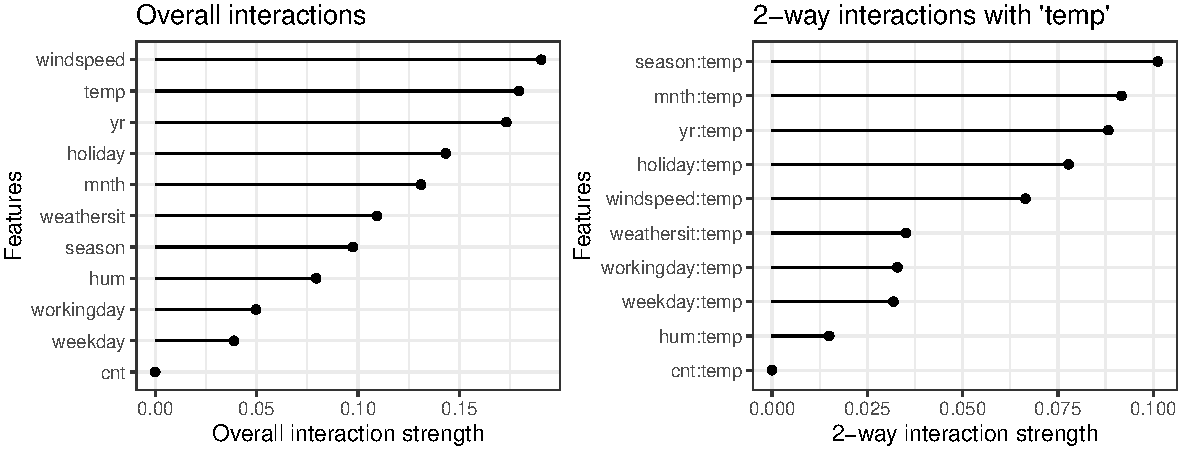
\includegraphics[width=\textwidth]{figure/h-statistic}
\end{center}

\pause
\textbf{Remarks and Conclusion:}
\begin{itemize}
    \item H-statistic provides \textbf{general definition of interactions} + an \textbf{algorithm for computation} \\
    Also adjustable to categorical / discrete features and / or function values
    \item For interaction order $k$ still needs $¸\approx 2^k$ PD-functions
    \item Statistical test for whether interactions are present using this statistic
\end{itemize}

\end{frame}

\endlecture
\end{document}
